% Copyright 2009 Steven Shiells
% Copyright 2009 Vincent Rahli
% Copyright 2010, 2011 John Pirie
% Copyright 2010, 2011, 2012 Heriot-Watt University
%
% Permission is granted to copy, distribute and/or modify this document
% under the terms of the GNU Free Documentation License, Version 1.3 or
% any later version published by the Free Software Foundation; with no
% Invariant Sections, no Front-Cover Texts, and no Back-Cover Texts.  A
% copy of the license is included in the section entitled "GNU Free
% Documentation License".

\documentclass{report}

% Usage: 
%
%   \DeclareSwitch{XXX}
%
% If \ifXXX is undefined, this is equivalent to:
%
%   \newif\ifXXX
%   \XXXfalse
%
% Otherwise it does nothing.

% This file may be loaded many times.  On the first time, we want to
% use \newcommand.  On subsequent occasions, we want to use
% \CheckCommand.

\@ifundefined{DeclareSwitch}{\newcommand}{\CheckCommand}
  {\DeclareSwitch}[1]
  {\@ifundefined{if#1}%
    {% First, allocate the new boolean switch.
     \expandafter\newif\csname if#1\endcsname
     % Then initialize it to false.
     \csname #1false\endcsname}%
    {% We should check here that it is a proper boolean, but that is difficult.
    }%
   \message{(if#1=if\csname if#1\endcsname true\else false\fi)}}


\usepackage{fullpage}
\usepackage{graphicx}
\usepackage{a4}
\setlength{\parskip}{10pt}

\usepackage[usenames,dvipsnames]{xcolor}
\usepackage[colorinlistoftodos, textwidth=20mm, shadow]{todonotes}
\newcommand{\warning}[2][] {\todo[color=red, inline]{Warning: #2}}
\newcommand{\note}[2][] {\todo[color=RoyalBlue, #1]{Note: #2}}

\DeclareSwitch{incolor} % true to have colors such as comments in color
\DeclareSwitch{comm}    % true to print display the comments


% my switches
\incolortrue
\commfalse

%%%%%%%%%%%%%%%%%%%%%%%%%%%%%%%%%%%%%%%%%%%%%%%%%%%%%%%%%%%%%%%
%%%%%%%%%%%%%%%%%%%%%%%%%%%%%%%%%%%%%%%%%%%%%%%%%%%%%%%%%%%%%%%
%%
%% Copyright 2009, 2010 Steven Shiells
%%
%% This file is free software: you can redistribute it and/or modify
%% it under the terms of the GNU General Public License as published by
%% the Free Software Foundation, either version 3 of the License, or
%% (at your option) any later version.
%%
%% This file is distributed in the hope that it will be useful,
%% but WITHOUT ANY WARRANTY; without even the implied warranty of
%% MERCHANTABILITY or FITNESS FOR A PARTICULAR PURPOSE.  See the
%% GNU General Public License for more details.
%%
%% You should have received a copy of the GNU General Public License
%% along with Skalpel.  If not, see <http://www.gnu.org/licenses/>.
%%
%%
%% Authors: Steven Shiells
%% Date: December 2009
%% Description: My macros file
%%
%%%%%%%%%%%%%%%%%%%%%%%%%%%%%%%%%%%%%%%%%%%%%%%%%%%%%%%%%%%%%%%%
%%%%%%%%%%%%%%%%%%%%%%%%%%%%%%%%%%%%%%%%%%%%%%%%%%%%%%%%%%%%%%%%


\usepackage{color}

% my colors

\definecolor{mygray}{gray}{0.4}
\definecolor{fkgray}{gray}{0.2}
\definecolor{dkgray}{gray}{0.1}
\definecolor{ltgray}{cmyk}{0, 0, 0, 0.11}


\ifincolor
\definecolor{mywhite}{cmyk}{0.01, 0, 0.06, 0}
\definecolor{myyellow}{cmyk}{0, 0, 1, 0}
\definecolor{myred}{cmyk}{0, 0.443, 0.443, 0.0}
\definecolor{myorange}{cmyk}{0, 0.5, 0.8, 0.0}
\definecolor{myred2}{cmyk}{0, 0.9, 0.7, 0.1}
\definecolor{myblue}{cmyk}{0.4, 0.4, 0, 0}
\definecolor{mygreen}{cmyk}{1, 0, 1, 0}
\definecolor{mypurple}{cmyk}{0, 0.276, 0, 0.133}
\definecolor{mygrey}{cmyk}{0, 0, 0, 0.255}
\definecolor{inboxcol}{cmyk}{0,0,0,0}
\definecolor{mypink}{cmyk}{0,0.102,0.102,0}
\definecolor{mylightblue}{cmyk}{0.112,0.112,0,0}
\definecolor{mylightgreen}{cmyk}{0.122, 0, 0.122, 0}
\definecolor{mylightpurple}{cmyk}{0.008, 0.127, 0, 0.016}
\else
\definecolor{mywhite}{cmyk}{0, 0, 0, 0.05}
\definecolor{myyellow}{cmyk}{0, 0, 0, 0.1}
\definecolor{myred}{cmyk}{0, 0, 0, 0.2}
\definecolor{myorange}{cmyk}{0, 0, 0, 0.28}
\definecolor{myblue}{cmyk}{0, 0, 0, 0.35}
\definecolor{mygreen}{cmyk}{0, 0, 0, 0.5}
\definecolor{mypurple}{cmyk}{0, 0, 0, 0.41}
\definecolor{inboxcol}{cmyk}{0,0,0,0}
\fi

\newcommand{\whitetext}[1]{\textcolor{mywhite}{#1}}
\newcommand{\blacktext}[1]{\textcolor{black}{#1}}
\newcommand{\redtext}[1]{\textcolor{myred}{#1}}
\newcommand{\bluetext}[1]{\ifincolor
                \textcolor{blue}{#1}
        \else
                \textcolor{myblue}{#1}
        \fi}
\newcommand{\orangetext}[1]{\textcolor{myorange}{#1}}
\newcommand{\purpletext}[1]{\textcolor{mypurple}{#1}}
\newcommand{\greentext}[1]{\textcolor{mygreen}{#1}}
\newcommand{\yellowtext}[1]{\textcolor{myyellow}{#1}}

% commands for comments

\newcommand{\codebody}[1]{{\tt\small\renewcommand{\arraystretch}{1}$$#1$$}}
\newcommand{\incodebody}[1]{{\tt\small\renewcommand{\arraystretch}{0.8}$\Bl#1\El$}}
\newcommand{\Bl}{\begin{tabular}[t]{@{}l@{}}}
\newcommand{\El}{\end{tabular}}
\newcommand{\Bi}{\begin{tabular}[t]{@{\quad}l}}
\newcommand{\Ei}{\end{tabular}}
\newcommand{\modifyboxdimen}[2]
  {% trashes \dimen0
   \dimen0=#1%
   \advance\dimen0 by #2%
   #1=\dimen0 % <- space is significant
  }

\newcommand{\examplebox}[2]
  {\begingroup
     \setbox0=\hbox{(g)}% use to determine standard height and depth
     \modifyboxdimen{\ht0}{0.5pt}%
     \modifyboxdimen{\dp0}{0pt}%
     \setbox1=\hbox{#2}%
     \ht1=\ht0%
     \dp1=\dp0%
     \setlength{\fboxsep}{0pt}% default 3pt
     \setbox2=\hbox{%\TraceExec
                    \colorbox{#1}{\box1}}%
                    % \colorbox{#1}{{\color{black}\box1}}}% only for talk
     %\bgroup
     % \tracingonline=1\relax
     % \showboxdepth=9999\relax
     % \showboxbreadth=9999\relax
     % \showbox2\relax
     %\egroup
     \modifyboxdimen{\ht2}{-0.5pt}%
     \modifyboxdimen{\dp2}{-0pt}%
     \box2%
   \endgroup}
\newcommand{\examplefbox}[2]
  {\begingroup
     \setbox0=\hbox{(g)}% use to determine standard height and depth
     \modifyboxdimen{\ht0}{0.5pt}%
     \modifyboxdimen{\dp0}{0pt}%
     \setbox1=\hbox{#2}%
     \ht1=\ht0%
     \dp1=\dp0%
     \setlength{\fboxrule}{1pt}% for talk only
     \setlength{\fboxsep}{0pt}% default 3pt
     \setbox2=\hbox{%\TraceExec
                    \fcolorbox{#1}{inboxcol}{\box1}}%
     %\bgroup
     % \tracingonline=1\relax
     % \showboxdepth=9999\relax
     % \showboxbreadth=9999\relax
     % \showbox2\relax
     %\egroup
     \modifyboxdimen{\ht2}{-0.5pt}%
     \modifyboxdimen{\dp2}{-0pt}%
     \box2%
   \endgroup}
\newcommand{\exampleffbox}[3]
  {\begingroup
     \setbox0=\hbox{(g)}% use to determine standard height and depth
     \modifyboxdimen{\ht0}{0.5pt}%
     \modifyboxdimen{\dp0}{0pt}%
     \setbox1=\hbox{#2}%
     \ht1=\ht0%
     \dp1=\dp0%
     \setlength{\fboxrule}{1pt}% for talk only
     \setlength{\fboxsep}{0pt}% default 3pt
     \setbox2=\hbox{%\TraceExec
                    \fcolorbox{#1}{#3}{\box1}}%
     %\bgroup
     % \tracingonline=1\relax
     % \showboxdepth=9999\relax
     % \showboxbreadth=9999\relax
     % \showbox2\relax
     %\egroup
     \modifyboxdimen{\ht2}{-0.5pt}%
     \modifyboxdimen{\dp2}{-0pt}%
     \box2%
   \endgroup}

\newcommand{\boxBl}[1]{\examplebox{black}{#1}}
\newcommand{\boxW}[1]{\examplebox{mywhite}{#1}}
\newcommand{\boxY}[1]{\examplebox{myyellow}{#1}}
\newcommand{\boxR}[1]{\examplebox{myred}{#1}}
\newcommand{\boxO}[1]{\examplebox{myorange}{#1}}
\newcommand{\boxB}[1]{\examplebox{myblue}{#1}}
\newcommand{\boxG}[1]{\examplebox{mygreen}{#1}}
\newcommand{\boxP}[1]{\examplebox{mypurple}{#1}}
\newcommand{\boxEnd}[1]{\examplebox{mygrey}{#1}}
\newcommand{\fboxBl}[1]{\examplefbox{black}{#1}}
\newcommand{\fboxW}[1]{\examplefbox{mywhite}{#1}}
\newcommand{\fboxY}[1]{\examplefbox{myyellow}{#1}}
\newcommand{\fboxR}[1]{\examplefbox{myred}{#1}}
\newcommand{\fboxB}[1]{\examplefbox{myblue}{#1}}
\newcommand{\fboxG}[1]{\examplefbox{mygreen}{#1}}
\newcommand{\fboxO}[1]{\examplefbox{myorange}{#1}}
\newcommand{\fboxP}[1]{\examplefbox{mypurple}{#1}}
\newcommand{\fboxEnd}[1]{\examplefbox{mygrey}{#1}}
\newcommand{\fboxGen}[3]{\exampleffbox{#1}{#2}{#3}} %% #1 colour outside, #2 text, #3 colour inside

\newcommand{\instruction}[1]{\incodebody{<{#1}>}}

\newcommand{\tesEndPointOne}[0]{gray }

\newcommand{\tesDownloadURL}[0]{\codebody{\Bl http://www2.macs.hw.ac.uk/{\textasciitilde}rahli/cgi-bin/slicer/downloads.html \El}}
\newcommand{\tes}[0]{type error slicer}
\newcommand{\tesing}[0]{type error slicing}
\newcommand{\Tesing}[0]{Type Error Slicing}
\newcommand{\Tes}[0]{Type Error Slicer}
\newcommand{\file}[1]{\textsf{#1}}


\title{Skalpel 0.8 User Guide}
\date{\today}

\begin{document}

\maketitle
\vspace{110mm}

\newpage

\tableofcontents

\newpage

\chapter {Installation}
\label{skalpel-installation}

This chapter will provide information on how the Skalpel packages and
archives can be installed.

\section {Skalpel Downloads Page}
\label{skalpel-downloads-page}

Installation packages and archives for Windows and Linux systems can
be found at the Skalpel downloads page (below):

\begin{center}\texttt{http://www.macs.hw.ac.uk/ultra/skalpel/downloads.html}\end{center}

\section {Linux}

Packages have been prepared for Debian and Red Hat based systems, and
can be found on the Skalpel downloads page (section
\ref{skalpel-downloads-page}). Readers who do not wish to install the
pre-prepared packages (for example those with other Linux
distributions or those who do not have root access will not be able to
install from these packages) should skip to section
\ref{archive-installation}, which discusses how to install Skalpel
from a tarball archive).

\subsection {Packages}

There are two different software packages available, the first is
\texttt{skalpel}, and the second is \texttt{skalpel-emacs}.

The \texttt{skalpel} package will install some crucial files (for
example the \texttt{skalpel} binary) and some documentation. This
package contains everything the user will need in order to run Skalpel
from a terminal window.

The \texttt{skalpel-emacs} package is an optional package that is
available for those that wish to use Emacs as a front-end to the
Skalpel program. Having the \texttt{skalpel} package installed is a
dependancy of this package.

Installation of the Red Hat based (.rpm) packages can be achieved by
running the below command as root:

\texttt{\# rpm -ivh $<$package\_name$>$}

Installation of the Debian packages can be achieved by running the
below command as root:

\texttt{\# dpkg -i $<$package\_name$>$}

\subsection {Archive Installation}
\label{archive-installation}

A \texttt{.tar.gz} archive has been prepared for users who for
whatever reason do not wish to use the Red Hat or Debian
packages. This archive in addition to containing crucial files (such
as the \texttt{skalpel} binary program) also contains the files
necessary to use Emacs as a front-end to Skalpl.

To install Skalpel from this archive, first download the tarball
(download link in section \ref{skalpel-downloads-page}), and extract
it using the command \texttt{tar -xzvf $<$filename$>$}.

Navigate into the extracted folder using \texttt{cd}.

Which command should be run next will depend on whether it is desired
that Skalpel is installed on the system for all users (requires root
permissions), or whether it is desired that Skalpel be installed in the
current user account only (does not require root permissions). To
install on the system for all users, run the following command:

\texttt{./configure}

Alternatively, if Skalpel is to be installed in the current user
account only, run the following command, replacing
$<$location$>$ with a directory path where Skalpel is to be installed:

\texttt{./configure --prefix=$<$location$>$}

If the configure script fails, either the prefix directory doesn't
already exist or the system does not have the necessary dependancies
to build Skalpel. Install all dependancies that were listed as missing
by the configure script and then run the configure script
again. Otherwise, if the configure script has succeeded, run
\texttt{make} (which will build the \texttt{skalpel} binary), followed
by \texttt{make install}, which will install the binary to the desired
location.

\section{Windows}

Simply double click on the executable file downloaded and the
installer program will launch, from there follow the instructions the
installer provides on the screen.

\chapter{Configuration of Front-Ends}

This chapter gives information on how to configure a system to use
Skalpel. Installation of Skalpel is covered in section
\ref{skalpel-installation}, and should be completed prior to reading
this section.

\section{Linux}

\subsection{Configuration of the Terminal Front-End}
\label{skalpel-environment-vars}

To use Skapel in a terminal, the analysis engine binary (the binary
installed to the system called \texttt{skalpel}), should be called
directly. There are a number of command-line options available, and
full list of these and an explanation for each can be found in section
\ref{command-line-arguments}, but the most important command line
arguments are as follows:

\begin{itemize}
\item \texttt{skalpel -b 2 $<$filename$>$:} This command line option
  specifies a file that Skalpel should choose to use as its
  basis file (this file contains definitions, such as the definition of the
  type list). A file is supplied with Skalpel in the likely event that the
  user does not wish to use their own, and the path to the
  \texttt{basis.sml} file supplied with Skalpel should go in place of
  $<$filename$>$ here.

  For users who are using the basis file that is supplied in the
  \texttt{skalpel} package/archive, it is recommended that the
  environment variable \$SKALPEL\_BASIS is set, which will allow the
  user to omit this argument. This can be done with similar lines to
  the below specified in the \texttt{{\textasciitilde}/.bashrc} file\footnote{ Users of shells
    other than bash should consult the documentation for their shell
    to discover how to set environment variables.}:\\

  \texttt{SKALPEL\_BASIS="/path/to/basis.sml"}\\
  \texttt{export SKALPEL\_BASIS}

\end{itemize}

The Skalpel program binary should also be added to the PATH variable
of the shell inside which Skalpel is to be executed. This can be
achieved as follows (users not using \texttt{bash} should consult the
documentation of their shell if they need to know how to do this),
replacing /path/to/dir/containing/skalpel/binary as appropriate:

\noindent \texttt{PATH=/path/to/dir/containing/skalpel/binary:\$PATH}\\
\texttt{export PATH}

\subsection{Configuration of the Emacs Front-End}

If the \texttt{skalpel-emacs} package (.rpm or .deb format) has been
installed then no configuration should be necessary. Otherwise, if the
Skalpel archive was downloaded from the downloads page (see
\ref{skalpel-downloads-page} for URL) then Emacs needs to be
configured to load an Emacs lisp file present inside the archive which
can be done by inserting the following lines into an Emacs startup
file\footnote{ Examples of startup files Emacs looks for include
  \texttt{{\textasciitilde}/.emacs} and
  \texttt{{\textasciitilde}/.emacs.el}}, replacing
/path/to/extracted/archive/ as appropriate:

\noindent \texttt{(add-to-list 'load-path (file-truename "/path/to/extracted/archive/front-ends/emacs/"))}\\
\texttt{(defvar skalpel-emacs-directory "/path/to/extracted/archive/front-ends/emacs/")}\\
\texttt{(defvar skalpel-bin-directory "/path/to/extracted/archive/analysis-engines/standard-ml/bin")}\\
\texttt{(defvar skalpel-lib-directory "/path/to/extracted/archive/lib/")}\\
\texttt{(defvar skalpel-sources-directory "/path/to/extracted/archive/analysis-engines/standard-ml/")}\\
\texttt{(load "skalpel-config.el")}

If configuration is set up correctly, the 'Skalpel' menu bar item will
be visible when in any file with the suffix ``.tes'', ``.sml'' or
``.sig.''.

\chapter{Using Skalpel in a Terminal Window}
\label{command-line-arguments}

For the purposes of this chapter, it is assumed that we have the
SKALPEL\_BASIS environment variable set up (described in section
\ref{skalpel-environment-vars}), and so the \texttt{-b} parameter is
omitted.

The skalpel analysis engine binary should be executed as follows:

\noindent \textbf{usage}: skalpel [option ...] [FILE]

where FILE is the file fed as input to be sliced. The command line
options and a description of each are as follows:

\
\begin{tabular}{|l|l|}
\indent \textbf{-l} $<$file$>$ & place output in $<$file$>$ in lisp format\\
\indent \textbf{-h} $<$file$>$ & place output in $<$file$>$ in HTML format\\
\indent \textbf{-s} $<$file$>$ & place output in $<$file$>$ in SML format\\
\indent \textbf{-j} $<$file$>$ & place output in $<$file$>$ in JSON format\\
\indent \textbf{-x} $<$file$>$ & place output in $<$file$>$ in XML format\\
\indent \textbf{-p} $<$file$>$ & place output in $<$file$>$ in perl format\\
\indent \textbf{-t} $<$timelimet$>$ & specify a numerical time limit\\
\indent \textbf{-x} $<$true/false$>$ & suppress exception handling (dev mode)\\
\indent \textbf{-c} $<$directory$>$ & Run analysis engine on tests in $<$directory$>$\\
\indent \textbf{-e} $<0\ |\ 1>$ & toggles echo of slice display in terminal (0=no, 1=yes)\\
\indent \textbf{-b} $<0\ |\ 1\ |\ 2 <$file$> >$ & Set basis level as 0 (no basis), 1 (built in basis), \\&2 $<$file$>$ (specify file as basis)\\
\indent -bo $<0\ |\ 1>$ & If set to 1, hides basis slice in overloading errors\\
\indent -tab $<$tabwidth$>$ & define the tab width in user code regions\\
\indent -sol $<$solution$>$ & define solution to use (default 9)\\
\indent -min $<$true/false$>$ & if true, shows non-minimal errors\\
\indent --print-env $<$true/false$>$ & whether to print the environment\\
\indent --show-legend & Shows the legend for notation and colour of slice display\\&in the terminal\\
\indent --search-space $<$1,2,3$>$ & Use search space 1 (lists), 2 (sets), or 3 (red black tree)\\
\indent --help & Show this help text
\end{tabular}

As an example, the user could execute this command in the terminal:

\textbf{skalpel -e 0 -p /tmp/test.pl -j /tmp/test.json /home/me/myfile.sml}

This would run Skalpel on the file /home/me/myfile.sml, with json and
perl slices being given as outut to /tmp, and the displaying of slices
in the terminal suppressed.

\chapter{Using Skalpel in Emacs}

\section{Running Skalpel}

%% \note{When running Skalpel, please ensure that all of
%%  the files you intend to run Skalpel on are saved -
%%  otherwise Skalpel will not execute.}

\subsection{Running Skalpel on a Single File}

\begin{itemize}
\item Open Emacs.
\item Load the SML file you wish to check.
\item From the \textbf{Skalpel} menu select the \textbf{Run Slicer}
  option (or alternatively press \texttt{F6}).
\end{itemize}

\subsection{Running Skalpel on Multiple Files}

\begin{itemize}
\item Open Emacs.
\item Load Skalpel control file (\texttt{.tes}) for
  the files you wish to check.\footnote{For the description of a type error slicer control file please read Section~\ref{sec:skalpel-control-files}.}
\item From the \textbf{Skalpel} menu select the \textbf{Run Slicer}
  option (or alternatively press \texttt{F6}).
\end{itemize}

%%%%%%%% VIEWING THE ERRORS %%%%%%%%

\section{Viewing the Errors}

Skalpel reports any errors by highlighting sections of
the source code. There may be multiple errors per file, some of which
may highlight parts of the source code that are also highlighted by
some other errors. In order to distinguish between the highlighting
of one error from another, the type error slice allows you to cycle
through all of the errors one at a time.

\subsection{View the Next Error Slice}

\begin{itemize}
\item From the \textbf{Skalpel} menu select the \textbf{Next Slice}
  option (or alternatively press \texttt{F7}).
\end{itemize}

\subsection{View the Previous Error Slice}

\begin{itemize}
\item From the \textbf{Skalpel} menu select the \textbf{Previous Slice}
  option (or alternatively press \texttt{F8}).
\end{itemize}

\subsection{Navigating Through the Different Parts of the Error Slice}
Type error slices may be quite large and may be at the opposite end of
a file, or in different files altogether. In these cases, it may not
be possible to view the whole slice all at the one time. In order to
determine what the problem is, it may be necessary to view all of
parts of the slice. Skalpel allows the user to cycle
through the different parts of the error slice that are not currently
in visible on screen. Details on how to use this feature can be seen below.

\begin{itemize}
\item From the \textbf{Skalpel} menu select the \textbf{Next Part of
  Slice} option (or alternatively press \texttt{Shift-F7}).
\end{itemize}

\subsection{Viewing the Details of the Error}

\begin{itemize}
\item Details of an error are automatically shown via a buffer which
  appears whenever the slicer is ran. If the user does not wish to see
  details of the error, they can disable this by unchecking the menu
  item \textbf{Skalpel $\rightarrow$ Slicing $\rightarrow$ Automatically display
    slice information}.
\end{itemize}

\section{Removing basis information during overloading errors}
\begin{itemize}
\item When encountering overloading errors, a lot of the information
  which is related to the errors lies in the basis. While this
  information is needed for correctness, there can be quite a lot of
  information to display and it is often of little help. In order to
  hide this information, make sure the \textbf{Type Error Slicing $\rightarrow$
    Slicing $\rightarrow$ Show basis information for overloading errors} checkbox
  is not ticked.
\end{itemize}

%%%%%%%% REMOVING THE HIGHLIGHTING %%%%%%%%

\section{Removing the Highlighting}

\subsection{Removing the Highlighting from the Current File}

\begin{itemize}
\item From the \textbf{Skalpel} menu select the \textbf{Remove
  Highlighting from Current File} option (or alternatively press
  \texttt{F9}).
\end{itemize}

\subsection{Removing the Highlighting from all Files}

\begin{itemize}
\item From the \textbf{Skalpel} menu select the \textbf{Remove
  Highlighting from all Files} option (or alternatively press
  \texttt{F10}).

  All highlighting in all the files are automatically removed each time
  Skalpel is run, allowing for the new highlighting to be displayed
  properly.

\end{itemize}

\section{Turn Verbose Error Messages On/Off}

Verbose error messages contain additional details of the errors which
may be useful for users who are not familiar with SML.  We allow users
to decide whether or not they wish to display these error messages.
Details of how to turn the verbose error messages on/off can be seen
below.  Note that verbosity of error messages only affect whether a
buffer includes explanations on the kind of the error in focus and
explanations on the colours used in the highlighting.

\subsection{Turning Verbose Error Messages On}

  \begin{itemize}
  \item From the \textbf{Skalpel}
    menu select the \textbf{Verbose Error Messages?} option.
  \end{itemize}

\subsection{Turning Verbose Error Messages Off}

  \begin{itemize}
  \item From the \textbf{Skalpel} menu
    deselect the \textbf{Verbose Error Messages?} option.
  \end{itemize}

%%%%%%%% MAKING THE SLICER EASIER TO USE %%%%%%%%

\section{Making Skalpel Easier to Use}

Key bindings can be set up that will allow the use of Skalpel without
the need to select menu items.  All of the code needed to do this is
supplied and can be found in the \texttt{skalpel-config.el} file in
the \texttt{front-ends/emacs/} folder.  For details on how to make the key
bindings active, please see Section~\ref{sec:setting-key-bindings}.

%%%%%%%% CREATING A TES CONTROL FILE %%%%%%%%

\section{Creating a Type Error Slicer Control File}
\label{sec:skalpel-control-files}

A type error slicer control file is a file that allows Skalpel to
slice multiple files. It is essentially a file that contains an
ordered list of files you wish to run the slicer on. The steps needed
to create a type error slicer control file are listed below.

\begin{enumerate}
\item Create a new file with the \texttt{.tes} extension.
\item Add a list of files to be checked - these files can either be
  SML (\texttt{.sml}) or other type error slicer control
  (\texttt{.tes}) files.

  The order in of files is important.  Please list all files which
  depend on other files \textbf{after} the files they depend on,
  otherwise some errors may not be found.  Listing files in the wrong
  order in a \texttt{.tes} file may also cause false errors to be
  found.

\item Save the file.
\end{enumerate}

\newpage

%%%%%%%%% PERSONALISING SKALPEL %%%%%%%%%%

\section{Personalising Skalpel}

%%%%%%%%% SETTING UP KEY BINDINGS %%%%%%%%%%

\subsection{Setting up Key Bindings}
\label{sec:setting-key-bindings}

Default key bindings are available for certain features of the type
error slicer. Our default key bindings are set up in the file
\texttt{emacs-config.el} (which can be found in the
\texttt{front-ends/emacs} in Skalpel directory) and are only active in
SML modes (the SML program editing mode and the mode for interacting
with a running SML implementation).

%% is all of the code you need to set up the
%% bindings, all you need to do is remove the appropriate comments and
%% change the key bindings if you so wish.

\medskip
An example of setting up a key-binding can be seen below.

In the file \texttt{emacs-config.el} there will be a number of
pieces of code that look like
\texttt{(define-key map [f6] 'skalpel-run-slicer-exec)}

To change this binding to for example \texttt{CONTROL-F6}, the code
between the square brackets would change. The binding would then be:

\texttt{(define-key map [C-f6] 'skalpel-run-slicer-exec)}

\medskip
Below is the part of our code which sets key bindings (extracted from
the \texttt{emacs-config.el} file):

\texttt{
  ;; Make "F6" run Skalpel.\\
  (define-key map [f6] 'skalpel-run-slicer-exec)\\
  ;; Make "F7" display the next error slice.\\
  (define-key map [f7] 'skalpel-next-slice)\\
  ;; Make "Shift-F7" display the next part of the slice currently in focus.\\
  (define-key map [S-f7] 'skalpel-next-part-of-slice)\\
  ;; Make "F8" display the previous error slice.\\
  (define-key map [f8] 'skalpel-prev-slice)\\
  ;; Make "F9" remove all of the error slices from the current file.\\
  (define-key map [f9] 'skalpel-forget-all-slices-file)\\
  ;; Make "F10" remove all of the error slices from all files.\\
  (define-key map [f10] 'skalpel-forget-all-slices)\\
  ;; Make "F11" display the help buffer.\\
  (define-key map [f11] 'skalpel-show-help))
}


\newpage

%%%%%%%%% CHANGING COLOURS %%%%%%%%%%

\subsection{Changing Colours}

In order to highlight the sections of source code we use a feature of
Emacs call ``faces''. A face can be used to change the way that text
can be displayed. We use a number of faces to display all of the
supported types of highlighting.

The default colours can be edited by using Emacs
\texttt{customize-faces} command and selecting the face you wish to
edit. A list of the faces that we use and an example of what they look
like can be seen below.

\medskip

\textbf{The list of faces used to highlight sections of source code in
  Emacs}

\begin{center}
  \begin{tabular*}{0.75\textwidth}{@{\extracolsep{\fill}}  l l}
    \multicolumn{1}{c}{\textbf{Name of Face}} &
    \multicolumn{1}{c}{\textbf{Example of Face}} \\
    skalpel-standard-error-focus &
    \texttt{\boxR{highlighted code}} \\
    skalpel-standard-error-non-focus &
    \texttt{\examplebox{mypink}{highlighted code}} \\
    skalpel-standard-error-box-focus &
    \texttt{\fboxR{highlighted code}} \\
    skalpel-standard-error-box-non-focus &
    \texttt{\examplefbox{mypink}{highlighted code}} \\
    skalpel-standard-error-head-focus &
    \texttt{\boxR{\whitetext{\textbf{highlighted code}}}} \\
    skalpel-end-point-one-focus &
    \texttt{\boxB{highlighted code}} \\
    skalpel-end-point-one-non-focus &
    \texttt{\examplebox{mylightblue}{highlighted code}} \\
    skalpel-end-point-one-box-focus &
    \texttt{\fboxB{highlighted code}} \\
    skalpel-end-point-one-box-non-focus &
    \texttt{\examplefbox{mylightblue}{highlighted code}} \\
    skalpel-end-point-one-head-focus &
    \texttt{\boxB{\whitetext{\textbf{highlighted code}}}} \\
    skalpel-end-point-two-focus &
    \texttt{\boxEnd{highlighted code}} \\
    skalpel-end-point-two-nonfocus &
    \texttt{\examplebox{ltgray}{highlighted code}} \\
    skalpel-end-point-two-box-focus &
    \texttt{\fboxEnd{highlighted code}} \\
    skalpel-end-point-two-box-nonfocus &
    \texttt{\examplefbox{ltgray}{highlighted code}} \\
    skalpel-end-point-two-head-focus &
    \texttt{\boxEnd{\whitetext{\textbf{highlighted code}}}} \\
    skalpel-merged-regions-focus &
    \texttt{\boxG{highlighted code}} \\
    skalpel-merged-regions-non-focus &
    \texttt{\examplebox{mylightgreen}{highlighted code}} \\
    skalpel-further-explanations-focus &
    \texttt{\boxP{highlighted code}} \\
    skalpel-further-explanation-non-focus &
    \texttt{\examplebox{mylightpurple}{highlighted code}} \\
    skalpel-further-explanations-box-focus &
    \texttt{\fboxP{highlighted code}} \\
    skalpel-further-explanation-box-non-focus &
    \texttt{\examplefbox{mylightpurple}{highlighted code}} \\
    skalpel-parsing-error-focus &
    \texttt{\boxY{highlighted code}} \\
    skalpel-parsing-error-non-focus &
    \texttt{\boxY{highlighted code}} \\
  \end{tabular*}
\end{center}

\textbf{NOTE:} The colours shown above may be inaccurate due to
differences in printers. For a more accurate representation please
refer to the PDF version of this document.

\newpage

%%%%%%%%% INTERPRETING THE SLICES %%%%%%%%%%

\chapter{Interpreting Type Error Slices}

Our type error slicer uses a colour coded system to distinguish
between the different components of the type error slices, and
recognises a number of different kinds of errors. This section
contains a brief description of the different kinds of error that the
type error slicer recognises, a description of the different kinds of
information provided by Skalpel when reporting errors
and finally, an example of how Skalpel highlights the
erroneous code for each of the kinds of errors that are picked up by
the slicer.

%%%%%%%%% KINDS OF ERRORS %%%%%%%%%%

\section{Brief Description of the Kinds of Type Errors}

This section contains a brief description of each of the different
kinds of type errors that Skalpel handles.

\begin{itemize}

\item Type Constructor Clash \subitem -- occurs
  when two type constructors are constrained to be equal but
  are not, for example, \texttt{int = bool}.
\item Arity Clash \subitem -- occurs when a sequence of length N is
  constrained to be equal to a sequence of length M where N $\neq$ M.
\item Record Clash \subitem -- occurs when two records are
  constrained to be equal but a label appears in one record and does
  not appear in the other.
\item Circularity Error \subitem -- occurs when a type is
  constrained to contain itself (an infinite type).
\item Inclusion Error \subitem -- occurs when there is a free type
  variable in a datatype or type declaration.
\item Multi-occurrence Error \subitem -- occurs when an identifier
  is bound more than once in one declaration.
\item Applied Value Variable Error \subitem -- occurs when a value
  variable is supplied an argument in a pattern.
\item Different Function Name Error \subitem -- occurs when a
  function is declared with 2 differing names.
\item Free Explicit Type Variable at Top Level Error \subitem --
  occurs when there is a type variable in the top level environment
  that is not bound to anything (free).
\item Value on the Left of \texttt{as} Error \subitem --
  occurs when the identifier on the left of an \texttt{as} is
  not a value variable.
\item An Identifier Occurs in a Pattern Both Applied and Not Applied to
  an Argument. \subitem -- occurs when the arity of an identifier is determined to be two different values.
\item Different Number of Arguments Error.  \subitem -- occurs when a
  function is defined to take an inconsistent number of arguments.
\item Ungeneralisable Bound Type Variable.  \subitem -- occurs when SML does
  not allow generalisation of type variables at certain value
  declarations.
\item Unmatched Specification Error. \subitem -- Occurs when a structure does not declare an identifier that it is supposed to..
\end{itemize}

\section{What the Colours Mean}

\begin{itemize}

\item \texttt{\boxR{Red}}

\begin{itemize}
\item Indicates that the highlighted text contributes to the error.
\end{itemize}

\item \texttt{\boxEnd{gray}/\boxB{blue}}

\begin{itemize}
\item Indicates that the highlighted text is an end point of a
  type constructor clash, an arity clash, or a record clash.

\end{itemize}

\item \texttt{\boxG{Green}}

\begin{itemize}
\item Indicates an endpoint of a record clash. The highlighted text
  appears in both clashing records. When there is green
  highlighting in a slice, it means that the slice merges at least two
  minimal slices.
\end{itemize}

\item \texttt{\fboxBl{Box}}

\subitem If the box is just an outline, with no colour inside the box,
  this signifies that the content of the box might be irrelevant, but its
  presence definitely contributes to the error.

\subitem If there is a colour in the box, then the
  content of the box is relevant to the error, and the reason why it
  is relevant is dependant on its colour (which are explained above).

\subitem A box can indicate one of two things:

\begin{enumerate}
\item The application of a
  function to an argument (the content of the box) takes part in an
  error. It is usually convenient to surround the argument of a
  function when the application participates in the error.
\item The contents of the box are the unique argument of a type name
  to make explicit its arity is 1 (that is, has one argument). This is
  because there is no section of code to highlight, making explicit the
  arity of a type name when its arity is 1.
\end{enumerate}

\item \texttt{\boxY{Yellow}}

\begin{itemize}
\item Indicates that Skalpel cannot parse the file. This
  may be because the file contains a feature of SML that has not yet
  been implemented in Skalpel, or, the file contains a
  syntax error.
\end{itemize}

\item \texttt{|\hspace{-0.03in}code}

\begin{itemize}
\item The use of a vertical bar (\texttt{|}) indicates an empty sequence of type
  arguments. \textbf{Note:} The colour of the vertical bar will be one of those
  above.

  For example, consider the following piece of code:

  \codebody{\Bl val x:t t = y \El}

  The slicer produces the following output:

  \codebody{\Bl \boxR{val} x:\fboxGen{mygray}{\hspace{-0.028in}\bluetext{|}\hspace{-0.03in}t}{myred}\boxR{ t} \boxR{=} y \El}

  The reason this is an error is that the first occurrence of t has no
  arguments, where as the second occurrence of t has one. The blue
  vertical bar is used to show that the first occurrence of t has no arguments
  and the \tesEndPointOne box is used to show the unique argument of the second
  occurrence of t.
\end{itemize}

\end{itemize}

\newpage

\section{Type Errors Explained (with examples)}

\subsection{Explanation of useful terms}
\begin{itemize}

%%%%%%%% TYPE ERROR SLICE %%%%%%%%%

\item Type Error Slice

  \subitem A type error slice is a piece of code that contains all of
  the points in a program that contribute to a type error with all of
  the other details omitted. In this document type error slices will
  normally be referred to as ``slices''.

%%%%%%% MINIMAL SLICE %%%%%%%%%%

\item Minimal Slice

  \subitem A minimal slice is an error slice which contains all of the
  program points that are required for the error to exist and nothing
  more.

%%%%%%% PROGRAMMING ERRORS %%%%%%%%

\item Programming Errors

  \subitem A programming error is an error which causes the program to
  do something other than it is meant to do. A programming error may
  or may not be responsible for type errors, but can contribute to an
  arbitrary number of type errors.

%%%%%%%% CONTEXT DEPENDENCY %%%%%%%%%

\item Context Dependencies

  \subitem In some of the errors reported by Skalpel, it
  will be only be an error if some identifiers are value variables,
  this is a context dependency: the error is dependent on the context
  of the identifier in a pattern.When there is not information to
  determine the true status of an identifier(s), Skalpel
  will report the error under the context dependency that the
  identifier is a value variable, as values in patterns are more often
  variables than constructors. If such a situation arises, then the
  error reported by Skalpel contain details of all
  context dependencies associated with the error.


%%%%%%%% TYPE ERRORS %%%%%%%%%%%%%%

\item Type Error

  \subitem For a program to be correctly typed, there is a number of
  constraints that have to be met. A type error occurs when all of
  these constraints cannot be satisfied simultaneously.

%%%%%%% TYPE CONSTRAINT %%%%%%%%%

\item Type Constraint

  \subitem A type constraint is when a value is constrained to be of a
  certain type, for example, in the piece of code below, \texttt{x} is
  constrained to be of type \texttt{bool}, \codebody{\Bl val x = true
    \El}

\newpage

%%%%%%%% TYPE CONSTRUCTOR CLASH %%%%%%%%%%%

{\large The rest of this section contains explanations of the type errors
recognised by Skalpel.}
\vspace{0.1in}
\subsection{Type Constructor Clash}

  \subitem A type constructor clash occurs when two type constructors
  are constrained (by the constraints mentioned previously) to be equal but
  they are not.

  For example, consider the following code.

\codebody{\Bl fun count x = x + true \El}

As one can see from the example, we have a \texttt{+} which is
an infix operator that represents numeric addition. One of the
arguments that is applied to this operator is \texttt{true}
which is a Boolean. As a Boolean is not a number and \texttt{+}
is not a Boolean operator, there is no way that this statement can be
assigned to have one type.

The slicer highlights the error in the following way:

\codebody{\Bl fun count x = x \boxB{+}\boxR{ }\boxEnd{true} \El}

As can be seen, the \texttt{+} operator has been highlighted in blue and
\texttt{true} in \tesEndPointOne. The differing colours indicate that
\texttt{true} and \texttt{+} are not of the same type,
thus causing an error.

\newpage

%%%%%%%%% ARITY CLASH %%%%%%%%%%%%%%%%%%%%%

\subsection{Arity Clash}

  \subitem An arity clash happens when a sequence of length N is
  constrained to be equal to a sequence of length M, where N $\neq$ M.

For example, consider the following piece of code.

\codebody{\Bl datatype 'a t = T of 'a t | U of ('a, 'a) t \El}

In the example above, \texttt{t} occurs with one argument,
\texttt{'a t}, as well as occurring with two arguments
\texttt{('a, 'a) t}. In this example, the slicer provides two
slices:

\codebody{\Bl datatype 'a t = T of \fboxB{'a}\boxR{ t} | U of
  \boxEnd{(}'a\boxEnd{,} 'a\boxEnd{)}\boxR{t} \El}

as well as

\codebody{\Bl \boxR{datatype} \fboxB{'a}\boxR{ t} \boxR{=} T of 'a
  t | U of \boxEnd{(}'a\boxEnd{,} 'a\boxEnd{)}\boxR{t} \El}

As can be seen from the slices, both occurrences of \texttt{'a
  t} have been highlighted, with the \texttt{'a} part being
highlighted with the use of a box, indicating that it is the unique
argument of \texttt{t}, with the \texttt{t} being
highlighted in red. In this case, the box is used to stress that
\texttt{t} takes one argument and also indicating that the name
of the type variable \texttt{'a} is irrelevant. In both slices,
the brackets and the comma of the section of code \texttt{('a,
  'a)t} have been highlighted in \tesEndPointOne, with the following
\texttt{t} again being highlighted in red. The \tesEndPointOne highlights
clearly show that the last occurrence of \texttt{t} is supplied
with two arguments. The user can therefore determine from both slices
provided that all occurrences of \texttt{t} should be supplied
with the same number of arguments but this is not the case.

In order to correct the error, the user can alter the code so that all
occurrences of \texttt{t} have the same number of arguments
(same arity).

\newpage

%%%%%%%%% RECORD CLASH %%%%%%%%%%%%%%%%%%%%%%%

\subsection {Record Clash}

\subitem A record clash occurs when two records are constrained to be
equal but a label appears in one record and does not appear in the other.
\\
For example, consider the following code:

\codebody{\Bl val \{foo,bar\} = \{fool=0,bar=1\} \El}

As can be seen, the label \texttt{foo} appears in the first record but does
not appear in the second one. Also the label \texttt{fool} appears in
the second record but does not appear in the first one. Hence, we have
a record clash. Skalpel returns the following output:

\codebody{\Bl \boxR{val}
  \boxR{\{}\boxB{foo}\boxR{,}\boxG{bar}\boxR{\} =
    \{}\boxEnd{fool}\boxR{=}0\boxR{,}\boxG{bar}\boxR{=}1\boxR{\}} \El}

The above example is actually two minimal slices merged together. With
this kind of error, merging the slices together makes the causes of
the error easier to identify. Finding record clashes can be time
consuming, so sometimes the merged slice will not be returned. The two
slices that are merged to make the slice above can be seen below.

\codebody{\Bl \boxR{val}
  \boxR{\{}\boxB{foo}\boxR{,}bar\boxR{\} =
    \{}\boxEnd{fool}\boxR{=}0\boxR{,}\boxEnd{bar}\boxR{=}1\boxR{\}} \El}

\codebody{\Bl \boxR{val}
  \boxR{\{}\boxB{foo}\boxR{,}\boxB{bar}\boxR{\} =
    \{}\boxEnd{fool}\boxR{=}0\boxR{,}bar\boxR{=}1\boxR{\}} \El}

In the first slice above, \texttt{foo} is highlighted in blue and all
the right hand side expression is highlighted in \tesEndPointOne. This
is because \texttt{foo} does not appear in the set on the right hand
side, \texttt{\{fool,bar\}}.

In the second slice above, \texttt{fool} is highlighted in
\tesEndPointOne and all of the labels in the left-hand side are
highlighted in blue. This is because \texttt{fool} does not appear
in the set on the left hand side, \texttt{\{foo,bar\}}.

As can be seen from the merged slice, the slicer highlights
\texttt{foo} in blue and \texttt{fool} in
\tesEndPointOne. This is a combination of the two minimal slices. The slicer
also highlights both occurrences of \texttt{bar} in
\tesEndPointOne. This is because it appears in both clashing records.

\newpage

%%%%%%%% CIRCULARITY ERROR %%%%%%%%%%%%%%%%%%%%%%

\subsection{Circularity Error}

\subitem Circularity errors occur when a type is constrained to
contain itself. This kind of error is best explained through the use
of an example.

Consider the following pieces of code:

\codebody{\Bl fun f () = f () \El}

and

\codebody{\Bl fun f () = f () () \El}

In the first piece of code, the function f has type:
\texttt{unit -> 'a}.  In the second piece of code, we assume
that the right hand side of the function is of type \texttt{'a}
then the second occurrence of \texttt{f} would be of type
\texttt{unit -> unit -> 'a} and the first occurrence of
\texttt{f} would be of type \texttt{unit -> 'a}

This means that:

\codebody{\Bl unit -> 'a =  unit -> unit -> 'a \\ 'a = unit -> 'a\El}

As a result of this:

 \codebody{\Bl 'a = unit -> unit -> 'a = unit -> unit -> unit ->
 unit -> 'a = ...\El}

This can be better viewed as a tree structure.

\begin{figure}[!h]
\begin{center}
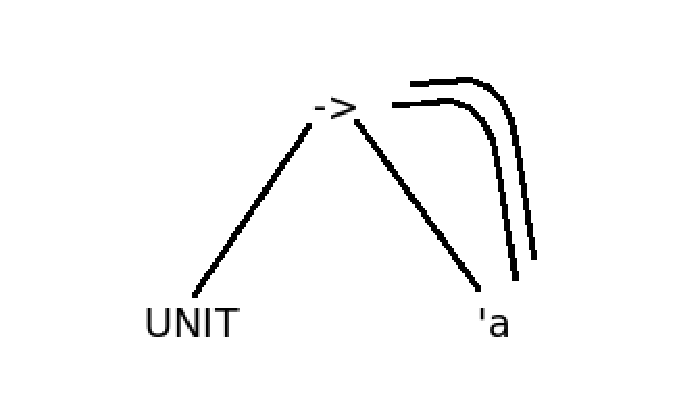
\includegraphics[scale=0.4]{tree.eps}
\end{center}
\end{figure}

As illustrated by the tree, the type of the function for the second
piece of code cannot be defined, as it would be assigned an infinite
type, which are not supported by SML, hence there is an error.

\newpage

%%%%%%%%% INCLUSION ERROR %%%%%%%%%%%%%%%%%

\subsection{Inclusion Error}

\subitem An inclusion error occurs when there is a free type variable
in a datatype declaration.

For example, consider the following piece of code:

\codebody{\Bl datatype 'a t = T of (bool -> ('a, 'b) w) \El}

The slicer highlights the code in the following way:

\codebody{\Bl \boxR{datatype} \boxR{'a }t \boxR{=} T of (bool ->
  ('a, \boxR{'b}) w) \El}

An important thing to notice here is that the slicer highlights the
space between \texttt{'a} and \texttt{t} in the
expression \texttt{datatype 'a t = ...}. This is to show that
it is the only type variable in the declaration of the datatype. The
occurrence of \texttt{'b} is also highlighted as
\texttt{'b} is the free
type variable that causes the error.

\vspace{1in}

%%%%%%%%%%%%% MULTI-OCCURRENCE ERROR %%%%%%%%%%%

\subsection{Multi-occurrence Error}

\subitem A multi-occurrence error occurs when an identifier is
declared twice in a unique declaration (binding).

For example, consider the following code:

\codebody{\Bl val (x, x) = (1, 1) \El}

Even though we are trying to assign the value \texttt{1} to
\texttt{x} twice, \texttt{x} appears more than once in
the pattern \texttt{val (x, x)} which is not permitted if x is
a value variable.

The slicer highlights the code in the following way (under the
context dependency that x is a value variable.

\codebody{\Bl \boxR{val} (\boxR{x}, \boxR{x}) \boxR{=} (1,1) \El}

As both occurrences of \texttt{x} are highlighted, and the fact
that this is a ``multi-occurrence'' error, the programmer can easily
see that the problem lies with the fact that there is more than one
occurrence of \texttt{x} is the reason behind the error. Also,
with the context dependency that \texttt{x} is value variable being
explicitly stated by the slicer, the programmer can then provide the
datatype defining \texttt{x} if his/her intentions were for
\texttt{x} to be a value constructor.

\newpage

%%%%%%%% APPLIED VALUE VARIABLE ERROR %%%%%%%%%%

\subsection{Applied Value Variable Error}

\subitem This error occurs when a value variable is supplied an
argument in a pattern.

For example, consider the following piece of code:

\codebody{\Bl val (x y, z, w) = (1, 2, 3) \El}

With the context dependency, \texttt{x} is a value variable,
 the slicer highlights the code as follows:

\codebody{\Bl \boxR{val} (\boxR{x }\fboxR{y}, z, w) \boxR{=} (1, 2,
  3)\El}

As \texttt{y} is highlighted by a box with a red line, it shows
that the content of the argument is irrelevant to the error, but the
presence of it is relevant. Going by the type of error and the context
dependency that \texttt{x} is a value variable, and the
application of \texttt{x} to an argument (\texttt{y}) is
highlighted, it is clear that the problem is caused by the mentioned
application, as SML does not allow value variables to be applied in a
pattern.

\textbf{Please Note:} this would not be the same error if x was a value
constructor (this is the reason the context dependencies of the error are
explicitly stated).

\vspace{0.5in}

%%%%%%% DIFFERENT FUNCTION NAME ERROR %%%%%%%

\subsection{Different Function Name Error}

  \subitem One of the constraints (we mentioned constraints in the
  section explaining type errors) that has to be met for a piece of
  code to be a valid SML program is that in a function definition,
  there must only be one name for the function.

Consider the following piece of code:

\codebody{\Bl fun count 0 = 1 | cout n = n + 1 \El}

As you can see in the code above, we have tried to give one function
two names. The slicer correctly identifies that this piece of code is
not correct and highlights it as follows:

\codebody{\Bl \boxR{fun} \boxR{count} 0 \boxR{=} 1 \boxR{|} \boxR{cout} n
  \boxR{=} n + 1 \El}

The slicer highlights \texttt{fun} which indicates that the
declaration of the function participates in the error. Both of the
names of the function are also highlighted. The equal signs and the
pipe character are also highlighted as they are essential parts of the
function definition. After a quick inspection of the slice, it becomes
easy to see that the function has two differing names, and the
programmer can correct the error accordingly.

\newpage

%%%%%%%%%% FREE EXPLICIT TYPE VARIABLE AT TOP LEVEL ERROR %%%%%%%%%%%%

\subsection{Free Explicit Type Variable at Top Level Error}

\subitem This error occurs when there is type variable in the top
level environment that is not bound to anything.

For example, consider the following piece of code:

\codebody{\Bl exception e of 'a \El}

The slicer highlights the code as (under the context dependency that
\texttt{'a} is at top level):

\codebody{\Bl \boxR{exception} e \boxR{of} \boxR{'a} \El}

The problem here is that \texttt{exception} does not implicitly
bind type variables.

\vspace{0.5in}

%%%%%%%% VALUE ON THE LEFT OF AS MUST BE A VALUE ERROR %%%%%%%%%%

\subsection{Value on the Left of ``as'' Must be a Variable Error}

\subitem No matter what the situation is, the identifier on the left
of an \texttt{as} must be a value variable, otherwise there is
a ``value on the left of \texttt{as} must be a value'' error.

Consider the following piece of code:

\codebody{\Bl datatype t = c; val c as (x, y) = (1, true) \El}

The problem here is that the identifier on the left of the
\texttt{as} (in this case \texttt{c}) is a value
constructor and not a value variable.

The slicer highlights the code as follows:

\codebody{\Bl \boxR{datatype} t \boxR{=} \boxR{c}; \boxR{val}
  \boxR{c as} (x, y) \boxR{=} (1, true) \El}

From the section \texttt{\boxR{datatype} t \boxR{=} \boxR{c}}
it can be seen that \texttt{c} is a value constructor. Using this
fact and the section \texttt{\boxR{val} \boxR{c as} ...} the
programmer can conclude that the error is caused by the use of a value
constructor on the left hand side of an \texttt{as} instead of
a value variable, and can go about correcting the error.

It should be noted that this error also occurs when the value on the
left hand side of the \texttt{as} is an exception constructor.
An example of an error involving this is shown below, along with the
highlighting produced by the slicer.

\codebody{\Bl exception e val e as x = 1; \El}

\codebody{\Bl \boxR{exception} \boxR{e} \boxR{val} \boxR{e as} x
  \boxR{=} 1; \El}

\newpage

%%%%%%%%%% AN IDENTIFIER OCCURS IN A PATTERN BOTH APPLIED AND NOT APPLIED

\subsection{An Identifier Occurs in a Pattern Both Applied and not Applied
  to an Argument}

\subitem This error is pretty self explanatory from the title, but the
reasons for such an error can be best explained through the use of an
example.

Consider the following piece of code:

\codebody{\Bl fn (f, f y, g x) => x + y \El}

The slicer highlights the code in the following way (the slicer
identifies other errors but this is the one we are interested in):

\codebody{\Bl \boxR{fn} (\boxR{f}, \boxR{f
  }\fboxR{y}, g x ) \boxR{=>} x + y \El}

As you can see, the slicer highlights both occurrences of
\texttt{f} with a solid red box, highlights
\texttt{y} with a clear box with a red outline and also
highlights the white space(s) between the occurrence of
\texttt{f} and its argument. This indicates
that the application of \texttt{f} to \texttt{y} is
significant in the error.

This error only occurs when the identifier appears inside a pattern
and can be caused by one of three things. The identifier in
question (in this case \texttt{f}) can either be:

\begin{enumerate}
\item A value variable --- in which case the identifier should not be
  applied to an argument,
\item A value constructor which is defined to take an argument --- in
  which case all occurrences of the identifier inside a pattern must take
  an argument, or
\item A value constructor which is defined to take no arguments --- in
  which case all occurrences of the identifier inside a pattern must take no arguments.
\end{enumerate}

%%%%%%% DIFFERENT NUMBER OF ARGUMENTS ERROR %%%%%%%%
\newpage

\subsection{Different Number of Arguments Error}

\subitem This error occurs when a function is defined to have an
inconsistent number of arguments.

Consider the following function declaration:

\codebody{\Bl fun foo 0 = 1 \\ \hspace{0.06in} | foo x y = x + y \El}

As you can see the function \texttt{foo} is defined to handle
both one argument and two arguments. This is not permitted in SML and
is therefore incorrect code. The slicer highlights the code as:

\codebody{\Bl \boxR{fun} foo\boxR{ }\fboxR{0}\boxR{ =} 1 \\
  \hspace{0.06in} \boxR{|} foo\boxR{ }\fboxR{x}\boxR{ }\fboxR{y}
  \boxR{=} x + y \El}
The slicer highlights the arguments of the function with a red
outline. This indicates that the presence of the arguments is
important in contributing to the error. Also, the slicer highlights
all of the code from the name of the function (\texttt{foo})
until \texttt{=} in the line(s) that contain less arguments
than the line(s) with the most. The reason for this is so that the
user can see all of the arguments in these lines and see that there
are not as many arguments on these lines as there are on other lines.
\textbf{Note:} The slicer is not implying that each of the lines in
the declaration should contain the same number of arguments as the
line that has the most, only that all lines should have the same number.

\subsection{Ungeneralisable Bound Type Variable Error}

\subitem Explicit type variables are usually generalisable at value
bindings but for some cases these type variables cannot be generalised
(due to some internal features of SML). These situations usually occur
when an explicit type variable occurs in the type of the bound
expression of a value declaration and this expression is expansive. It is
in these situations that a \texttt{Ungeneralisable Bound Type
  Variable Error} occurs.

An example of one of these situations can be seen below.

\codebody{\Bl val x = (fn y => fn x : \hspace{-0.1in}'a => x) [\hspace{0.05in}] \El}

The error occurs because the expression on the right hand side of the
\texttt{=} is expansive (application of an \texttt{fn} expression) and when you apply the function
\texttt{y} to the empty list (\texttt{[]}) you get a function
from type \texttt{'a} to type \texttt{'a} and the type
\texttt{'a} cannot be generalised.

The slicer highlights the error in the following way.

\codebody{\Bl \boxR{val} \boxR{x = (fn} y \boxR{=> fn} x \boxR{: \hspace{-0.1in}'a =>} x\boxR{) }\fboxR{[\hspace{0.05in}]} \El}

\newpage

%%%%%%% UNMATCHED SPECIFICATION ERROR %%%%%%%%

\subsection{Unmatched Specification Error}

\subitem This kind of error occurs when a structure does not declare
an identifier that it is supposed to.

Consider the following example:
\codebody{\Bl structure foo = struct val x = () end; \\ foo.y;\El}
There is an error in the above code because the structure
\texttt{foo} does not declare the identifier \texttt{y}.
The slicer highlights the code as:
\codebody{\Bl \boxR{structure} \boxR{foo} \boxR{=} \boxR{struct} \boxR{val} \boxR{x = }() \boxR{end}; \\ \boxR{foo.y};\El}

\end{itemize}

\chapter {Credits}
Vincent Rahli: Type Error Slicer Theory and Implementation.\\\\
Joe Wells: Theory and Implementation, Consulting Advice and Emacs
Interface.\\\\
John Pirie: Type Error Slicer Theory and Implementation.\\\\
Scott Fotheringham: Setup of Bugzilla and Emacs Interface\\\\
Mark Wyper: Testing of the effectiveness of Skalpel.\\\\
Steven Shiells: Web Interface Implementation and Emacs Interface.\\\\
David Dunsmore: Testing of the effectiveness of Skalpel.\\\\
Fairouz Kamareddine: Theory Consulting\\\\
Christian Haack: Type Error Slicer Theory and Implementation.\\\\
S\'ebastien Carlier: Web Interface Implementation.
\end{document}
